\chapter{Implementacija metod}
V tem poglavju so opisane implementacije nekaterih metod, opisanih v poglavju~\ref{sec:metode}. Gre za tiste metode, kjer iz teoretične podlage implementacija ni bila točno razvidna. Opisane so tudi metode, kjer teoretične podlage nismo podrobneje opisovali.

\subsection{Optični in prostorski tok}
Na podlagi opisanih lastnosti metod optičnega toka v poglavju~\ref{sec:metode-of} smo se odločili, da bomo v tem delu uporabili diferencialno metodo. Kljub višji računski zahtevnosti, ki ob današnji tehnologiji ne predstavlja več takega problema, smo želeli računati gost optični tok. Z gostim optičnim tokom dobimo natančno aproksimacijo polja gibanja za celotno telo. Prav tako nimamo problemov pri estimaciji energijske porabe za hitre gibe, kot bi bilo to v primeru uporabe ujemalnih metod. Ker je glavni namen uporaba in ne implementacija diferencialne metode, smo se osredotočili na Farneb{\"a}ck algoritem, ki je dostopen v knjižnici OpenCV 3.1.0.

Za optični tok smo uporabili sledeče parametre: piramidna skala $pyr\_scale=\num{0.5}$, število piramidnih slojev $levels=3$, velikost okna povprečenja $winsize=15$, število iteracij na vsakem piramidnem sloju $iterations=3$, velikost okolice slikovnih elementov $poly\_n=5$ in Gaussov standardni odklon $poly\_sigma=\num{1.2}$.

Z uporabo prostorskega toka lahko bolje opišemo mehanično delo kot pri uporabi optičnega toka. Vsekakor pa potrebujemo dodatno informacijo, ki jo moramo pridobiti iz slikovnih podatkov. Za ta namen smo uporabili kamere na podlagi časa preleta (ToF), ki so vgrajene v poceni senzor Microsoft Kinect for Windows V2~\cite{Yang2015KinectV2}. Z njim pridobivamo registrirane RGB-D (rdeče, zelene, modre in globinske) podatke. Za pridobitev prostorskega toka smo uporabili algoritem PD-Flow. Njegova implementacija je javno dostopna~\cite{jaimez2015primal}. Podrobneje je opisan v poglavju~\ref{sec:pd-flow}.



\subsection{Sledilniki}
Pri izbiri sledilnikov smo se osredotočili na pogoje, ki jim morajo sledilniki v največji meri zadostiti. Sledilnik mora dobro slediti osebam, ostali objekti niso pomembni. Sledenje mora biti zanesljivo, saj je od njega odvisna merilna napaka. Pri tem moramo upoštevati delovanje tudi v primerih, kadar tarča izgine iz slike. Sledenje mora delovati čim daljši čas tako, da ne potrebujemo ponovne inicializacije. Inicializacijo sledilnika moramo opraviti samo na prvi sliki zaporedja, kar pomeni, da mora sledilnik vsebovati indirektno učenje (angl. offline training). Zaradi uporabe sledilnika v merilnem instrumentu mora ta delovati čim hitreje. Ker namen tega dela ni implementacija sledilnika, mora biti ta implementiran v prosto dostopni izvorni kodi. 

Pri uporabi optičnega toka smo najprej preizkusili sledilnik TLD avtorja Kalal et al.~\cite{kalal2012tracking}. Prosto dostopne so tri implementacije sledilnika, in sicer v knjižnici ccv (CCV-TLD), v knjižnici OpenCV (OPENCV-TLD) in c++ izvorna koda (NEBEHAY-TLD). Implementaciji iz knjižnic ccv in OpenCV se nekoliko razlikujeta od izvirnega dela~\cite{kalal2012tracking}, NEBEHAY-TLD pa je samo prepis Matlabove izvorne kode.  Ker ni nobena implementacija zadovoljivo delovala na testnih squash posnetkih, smo poskusili še s sledilnikoma KCF~\cite{danelljan2014adaptive} in DLIB-CORR~\cite{danelljan2014accurate}. KCF je implementiran v knjižnici OpenCV, DLIB-CORR pa v knjižnici Dlib~\cite{king2009dlib}.

Testiranje sledilnikov je opisano v poglavju~\ref{sec:testiranje-sledilnikov-za-opticni-tok}, rezultati pa v poglavju~\ref{sec:rezultati-sledilnikov-za-opticni-tok}. Ugotovili smo, da najbolje deluje sledilnik KCF. Tega smo tudi uporabili v naših nadaljnjih eksperimentih.

Pri uporabi prostorskega toka smo preizkusili in uporbili sledilnik DS-KCF avtorja Hannuna et. al~\cite{hannuna2016ds}. Sledilnik uporablja RGB in globinske slike.


Rezultat sledenja je pri obeh uporabljenih sledilnikih (KCF in DS-KCF) okvir opazovanega subjekta. Notranjost okvirja uporabljamo za zapolnitev histogramov v deskriptorjih, preostanek toka v prizorišču zavržemo. Algoritma sledenja smo potrebovali za terenske teste, kjer položaj igralca ni znan. Kljub skrbni izbiri algoritmov je to najmanj robusten del našega pristopa---če sledilnik za posamezen časovni interval ne detektira igralca, manjkajo podatki na tem intervalu, razen če smo sledenje nadzorovali in odpravljali napake. Sledilnik ne detektira igralca kadar:

\begin{itemize}
	\item{Algoritem signalizira, da ni zaznal tarče.}
	\item{Algoritem signalizira nizko zaupanje v rezultat (predvsem zaradi okluzij).}
	\item{Površina področja tarče je 0.}
	\item{Vsi vektorji optičnega ali prostorskega toka so ničelni znotraj področja tarče.}
\end{itemize}

Naš pristop je dovolj modularen, da lahko enostavno zamenjamo algoritme za sledenje. S kakršnimi koli napredki na področju vizualnega sledenja se bo zanesljivost naše metode izboljšala.

\subsection{Kalmanov filter}\label{sec:implementacija-kalman}
Za prostor stanj smo izbrali stanje hitrosti $v$ in pospeška $a$~\eqref{eq:stanje}. 

\begin{equation}
\vec{x}(k) = \begin{bmatrix}
					v(k) & a(k)
				\end{bmatrix}^\top 
                \label{eq:stanje}
\end{equation}

Matrika prehajanja stanj je določena z enačbo~\eqref{eq:a}.

\begin{equation}
\vec{A} = \begin{bmatrix}
				1 & 1 \\
                0 & 1
			\end{bmatrix} 
            \label{eq:a}
\end{equation}

Za matriko vhodnih stanj $G$ smo izbrali~\eqref{eq:g}, s katero modeliramo neznane vhodne parametre hitrosti $v_n$ in pospeška $a_n$ v vektorju $u$~\eqref{eq:u}. 

\begin{equation}
\vec{G} = \begin{bmatrix}
				1 & 0
			\end{bmatrix}^\top 
            \label{eq:g}
\end{equation}

\begin{equation}
\vec{u}(k) = \begin{bmatrix}
					v_{n}(k) & a_n(k)
				\end{bmatrix}^\top 
                \label{eq:u}
\end{equation}


Merilna matrika je predstavljena z enačbo~\eqref{eq:h}
\begin{equation}
\vec{H} = \begin{bmatrix}
				1 & 0
			\end{bmatrix}^\top 
            \label{eq:h}
\end{equation}

Za začetno hitrost in pospešek smo izbrali vrednost $0$, ker se naši testi večinoma začnejo v mirovanju. 

Variance šuma modela gibanja, merilnega modela in kovariančne matrike stanja smo določili z uporabo mrežnega iskanja, ki je opisan v poglavju~\ref{sec:optimizacija-svm-parametrov}. Pri tem smo uporabili labele učnih vzorcev vseh testov 1. sklopa eksperimentov za referenco, njihove pošumljene ocene pa za meritev. Varianca šuma merilnega modela je tako znašala $\sigma_\vec{z}^2 = \num{0.04}$, varianca šuma modela gibanja pa $\sigma_\vec{x}^2 = \num{456.13}$. Za kovariančno matriko predikcije smo uporabili varianco $\sigma_\vec{P}^2 = \num{456.13}$. Kovariančno matriko modela gibanja smo določili po enačbi~\eqref{eq:Q}, kovariančna matrika merilnega modela je bila določena z enačbo~\eqref{eq:R} in začetna vrednost kovariančne matrike stanja z~\eqref{eq:P}.

\begin{equation}
\vec{Q} = \vec{G} \vec{G}^\top \sigma_\vec{x}^2
\label{eq:Q}
\end{equation}

\begin{equation}
\vec{R} = \sigma_\vec{z}^2
\label{eq:R}
\end{equation}

\begin{equation}
\vec{P}(0) = \begin{bmatrix}
1 & 0 \\
0 & 1
\end{bmatrix} \sigma_\vec{P}^2
\label{eq:P}
\end{equation}










\subsection{Gaussov filter}\label{sec:implementacija-gauss}

Gaussov filter smo implementirali po enačbi~\eqref{eq:gauss}. Za velikost jedra smo določili $3\sigma$, pri čemer je standardni odklon $\sigma$ parameter. Jedro smo nato še normirali na vsoto $1$. 

Za filtriranje podatkov smo uporabili modificirano Matlabovo funkcijo \texttt{nanconv}, ki je podrobneje predstavljena v~\cite{kraus2017nanconv}. Namesto funkcije \texttt{conv2} smo v modifikaciji uporabili funkcijo \texttt{conv}.






\subsection{Združevanje slik iz dveh Kinect kamer}
Zaradi ozkega vidnega polja Kinect kamer smo za pokritje celotne širine igrišča potrebovali dve kameri. Zaporedja slik smo pred nadaljnjo obdelavo morali združiti v eno zaporedje glede na opazovanega igralca. Zajem iz posameznih kamer ni bil sinhroniziran, zato smo pred združevanjem sinhronizirali posnetka tako, da smo izbrali slike iz posameznega zaporedja z najbolj podobnimi časovnimi žigi. Časovno sinhornizirana zaporedja slik smo nato poskušali združiti s tremi različnimi metodami:  združevanje z značilkami, združevanje s kontrolnimi točkami in prilagojeno združevanje. 

Časovno sinhronizirana zaporedja slik smo naprej poskušali združiti z metodo panoramskega šivanja slik z uporabo značilk, kot je opisano v delu~\cite{brown2007automatic}. Tu smo namesto SIFT značilk uporabili SURF značilke.
Združevanje s značilkami se ni obneslo, zato smo to metodo opustili. Primer neuspelega poskusa je prikazan na sliki~\ref{fig:zdruzevanje-znacilke}.

\begin{figure}[!htb]
	\centering
	\begin{subfigure}[t]{0.45\columnwidth}
		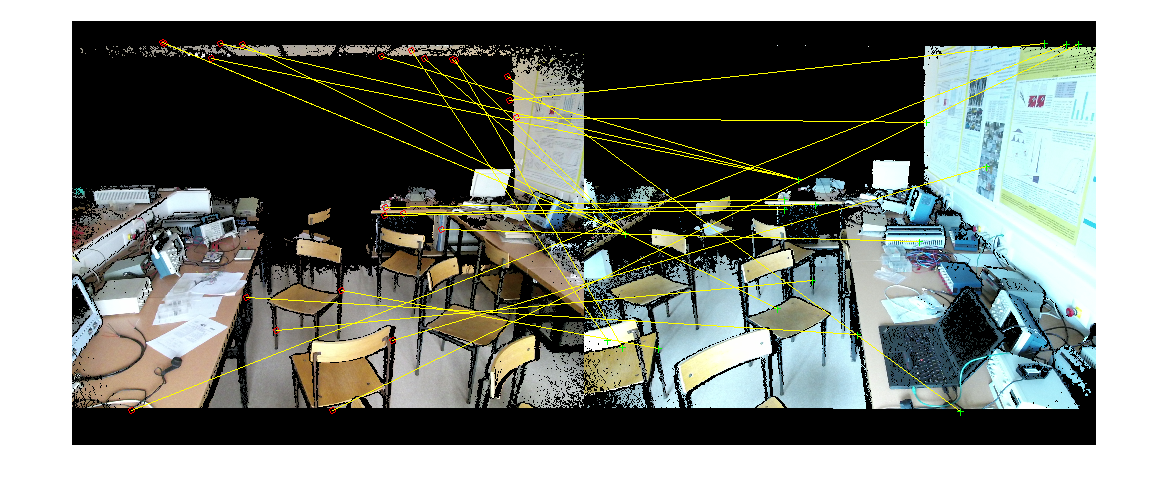
\includegraphics[width=\columnwidth]{./Slike/matched-features.png}
		\caption{Ujemajoče SURF značilke}
		\label{fig:zdruzevanje-surf}
	\end{subfigure}
	~
	\begin{subfigure}[t]{0.45\columnwidth}
		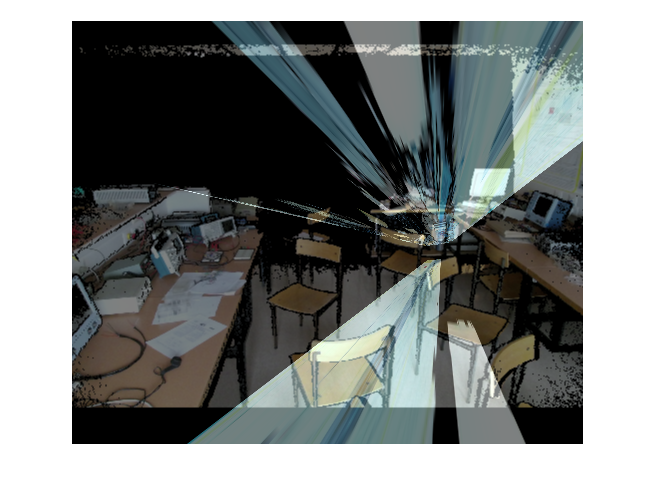
\includegraphics[width=\columnwidth]{./Slike/features-calibration-result.png}
		\caption{Rezultat združevanja z značilkami}
		\label{fig:zdruzevanje-result}
	\end{subfigure}
	\caption[Neuspelo združevanje slik s SURF značilkami]{Primer neuspelega poskusa združevanja slik iz dveh Kinect kamer s SURF značilkami.}
	\label{fig:zdruzevanje-znacilke}
\end{figure}

Zaporedja slik smo poskušali združiti tudi z ročnim določevanjem kontrolnih točk. Rezultat {združevanja s kontrolnimi točkami} je bil boljši od združevanja z značilkami, vendar še vedno slab, zato smo tudi to metodo opustili. Primer neuspelega poskusa je prikazan na sliki~\ref{fig:zdruzevanje-cp}.

\begin{figure}[!htb]
	\centering
	\begin{subfigure}[t]{0.45\columnwidth}
		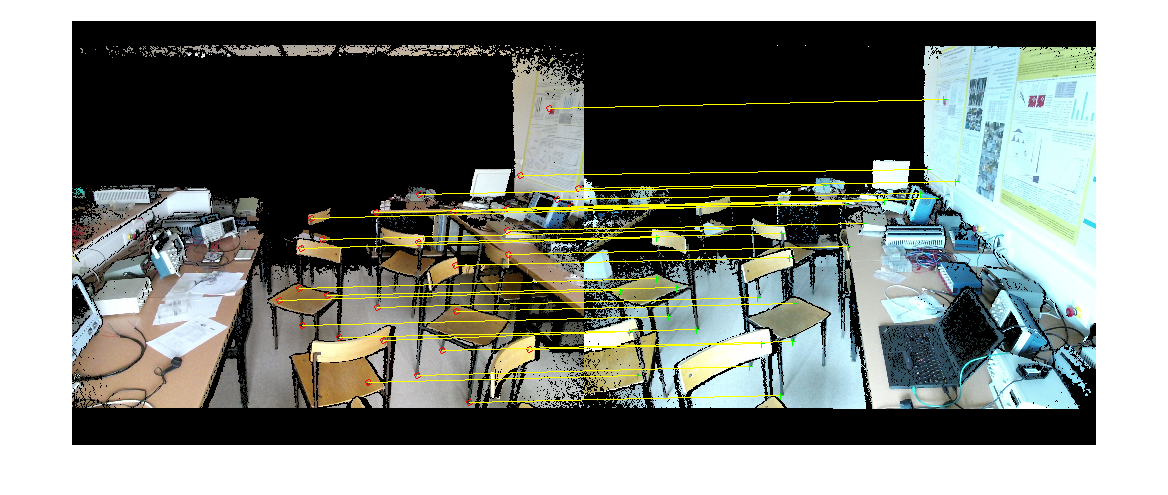
\includegraphics[width=\columnwidth]{matched-points.png}
		\caption{Ujemajoče kontrolne točke}
		\label{fig:zdruzevanje-ujemajoce-cp}
	\end{subfigure}
	~
	\begin{subfigure}[t]{0.45\columnwidth}
		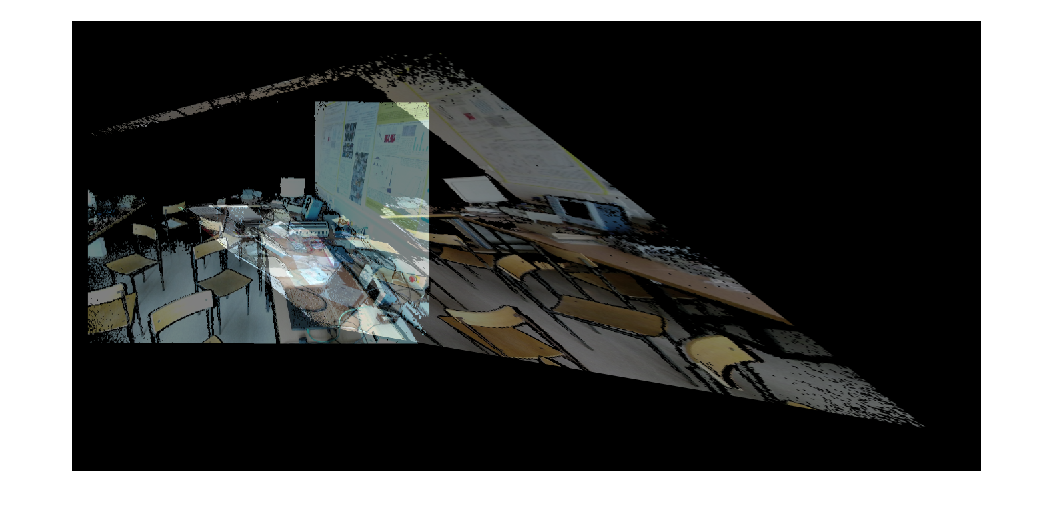
\includegraphics[width=\columnwidth]{points-calibration-result.png}
		\caption{Rezultat združevanja s kontrolnimi točkami}
		\label{fig:zdruzevanje-result-cp}
	\end{subfigure}
	\caption[Neuspelo združevanje slik s kontrolnimi točkami]{Primer neuspelega poskusa združevanja slik iz dveh Kinect kamer s kontolnimi točkami.}
	\label{fig:zdruzevanje-cp}
\end{figure}

Zaradi nezadovoljivih rezultatov klasičnih metod združevanja stereo slik smo razvili metodo, ki je prilagojena za Kinect kamere. Iz kamer smo z uporabo knjižnice libfreenect2 0.2~\cite{lingzhu2016libfreenect2} pridobili intrinzične parametre bližnje-infrardečega (NIR) senzorja, in sicer: slikovni koordinati goriščne razdalje $f_u$ in $f_v$ ter slikovni koordinati optičnega središča slike (ang. principal point) $c_u$ in $c_v$. Intrinzične parametre smo uporabili za določitev intrinzične matrike $\vec{M}_{int}$ po enačbi~\eqref{eq:intrinsic}.

Ker pravih ekstrinzičnih parametrov kamer nismo poznali, smo jih le ocenili z metodo določevanja sečišča vidnih polj obeh kamer. Sečišče je prikazano kot rdeča linija na sliki~\ref{fig:zdruzevanje}. S to metodo smo določili translacijski vektor $\vec{t} = \left [ t_x~ t_y~ t_z \right]^\top$ in rotacijsko matriko $\vec{R}$ iz Eulerjevih kotov.

S sledenjem igralca z DS-KCF algoritmom smo s pomočjo projekcijske matrike~\eqref{eq:projection-matrix} določili center tarče v metričnih enotah za vsako sliko zaporedja leve in desne kamere. Če center tarče ni vseboval podatkov globine, smo za center izbrali najbližjo točko z veljavno globino.

Prva slika združenega zaporedja je bila slika kamere, kjer se igralec prvič pojavi. Nadaljnje slike smo izbirali med zaporedjema kamer, glede na pozicijo centra tarče s histerezo, ki je na sliki~\ref{fig:zdruzevanje} prikazana z modrimi linijami. Pogled spremenimo samo takrat, ko center tarče prečka linijo histereze na igrišču. Razdalja med modrima črtama je znašala \SI{400}{mm}.


\begin{figure}[!htb]
	\centering
	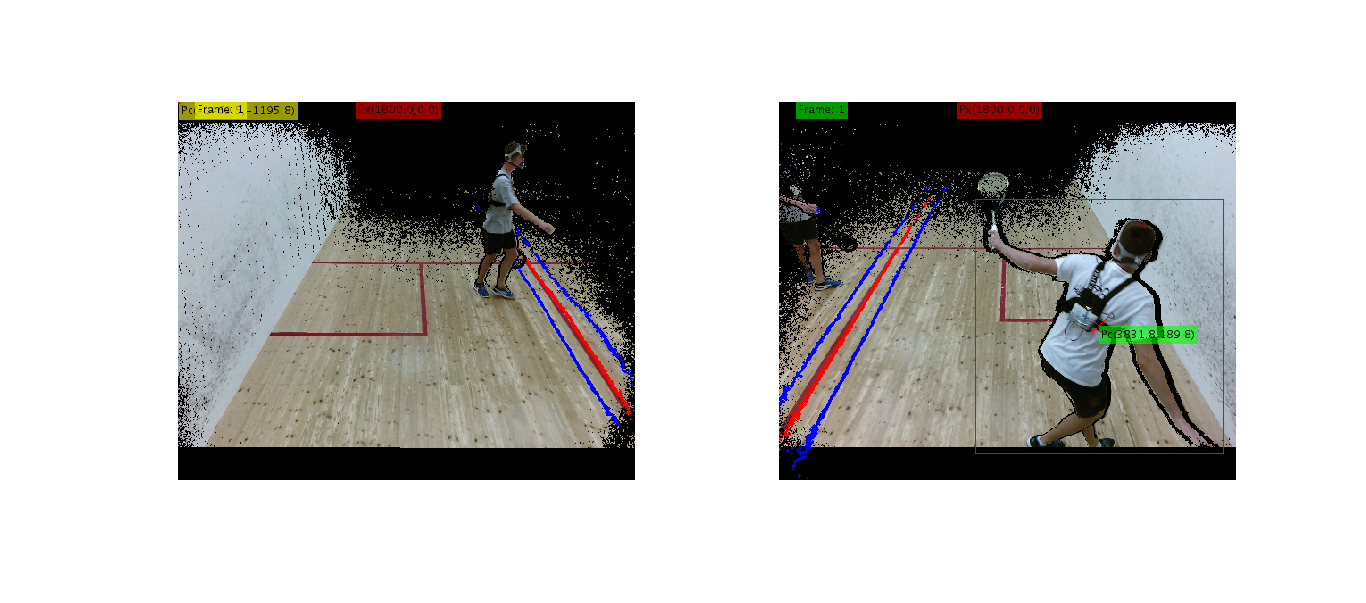
\includegraphics[width=\columnwidth]{zdruzevanje-example.png}
	\caption[Določevanje sečišča vidnih polj leve in desne Kinect kamere]{Določevanje sečišča vidnih polj leve in desne Kinect kamere. Na sliki sta prikazani prvi sliki zaporedja leve in desne Kinect kamere 1. seta 2. igre terenskega eksperimenta iz 2. faze. Označen je 4. igralec. Zelena barva koordinat centra tarče predstavlja izbrano kamero. Kamera z rumeno barvo ni izbrana. Sečišče je rdeča linija. Modri liniji sta pragova za preklop med kamerama. Razdalja med njima je \SI{400}{mm}.}
	\label{fig:zdruzevanje}
\end{figure}

